%----------------------------------------------------------------------------------------
%	PACKAGES AND OTHER DOCUMENT CONFIGURATIONS
%----------------------------------------------------------------------------------------

\documentclass{beamer}

\usetheme{focus} % Use the Focus theme supplied with the template
% Add option [numbering=none] to disable the footer progress bar
% Add option [numbering=fullbar] to show the footer progress bar as always full with a slide count

% Uncomment to enable the ice-blue theme
%\definecolor{main}{RGB}{92, 138, 168}
%\definecolor{background}{RGB}{240, 247, 255}

%------------------------------------------------

\usepackage{subfig}

\usepackage{booktabs} % Required for better table rules

\usepackage[brazilian]{babel}
\usepackage[utf8]{inputenc}
\usepackage[T1]{fontenc}

%----------------------------------------------------------------------------------------
%	 TITLE SLIDE
%----------------------------------------------------------------------------------------

\title{Diagnóstico do Glaucoma Usando Imagens de Espessura da Camada de Fibras Nervosas}

% \subtitle{VII Workshop de Pós-Graduação - Engenharia da Computação - WPGEC 2018}

\author{Samira J. Braga \\ Edson S. Gomi}

% \titlegraphic{\includegraphics[scale=1.25]{Images/focuslogo.pdf}} % Optional title page image, comment this line to remove it

\institute{Escola Politécnica da Universidade de São Paulo}

\date{22/11/2018}

%------------------------------------------------

\begin{document}

%------------------------------------------------

\begin{frame}
	\maketitle % Automatically created using the information in the commands above
\end{frame}

%----------------------------------------------------------------------------------------
%	 SECTION 1
%----------------------------------------------------------------------------------------

% \section{Objetivos e motivação} % Section title slide, unnumbered

%------------------------------------------------

\begin{frame}{Objetivo e motivação}
    Glaucoma é uma doença de difícil diagnóstico que pode levar à cegueira, se não tratada.
    
    O objetivo deste trabalho é investigar se é possível fazer o diagnóstico a partir das imagens da espessura da camada de fibras nervosas do olho por meio de uma rede neural convolucional (CNN).

    \begin{figure}
        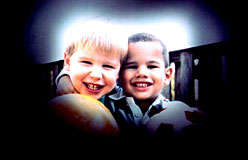
\includegraphics[width=1.5in]{img/glaucomavision.jpg} 
        \caption{Visão de uma pessoa com glaucoma}
    \end{figure}

\end{frame}

\begin{frame}{Diagnóstico do glaucoma}
    \begin{columns}
        \column{0.6\textwidth}
        
        \begin{itemize}
            \item  O  diagnóstico  do  glaucoma  é  feito  com  uma combinação  de  exames de OCT e perimetria  computadorizada
            \item Muitas vezes é necessária a avaliação de um especialista
            \item É possível utilizar algoritmos classificadores para auxiliar o oftalmologista na tomada de decisão
        \end{itemize}    

        \column{0.4\textwidth}
            \begin{figure}
                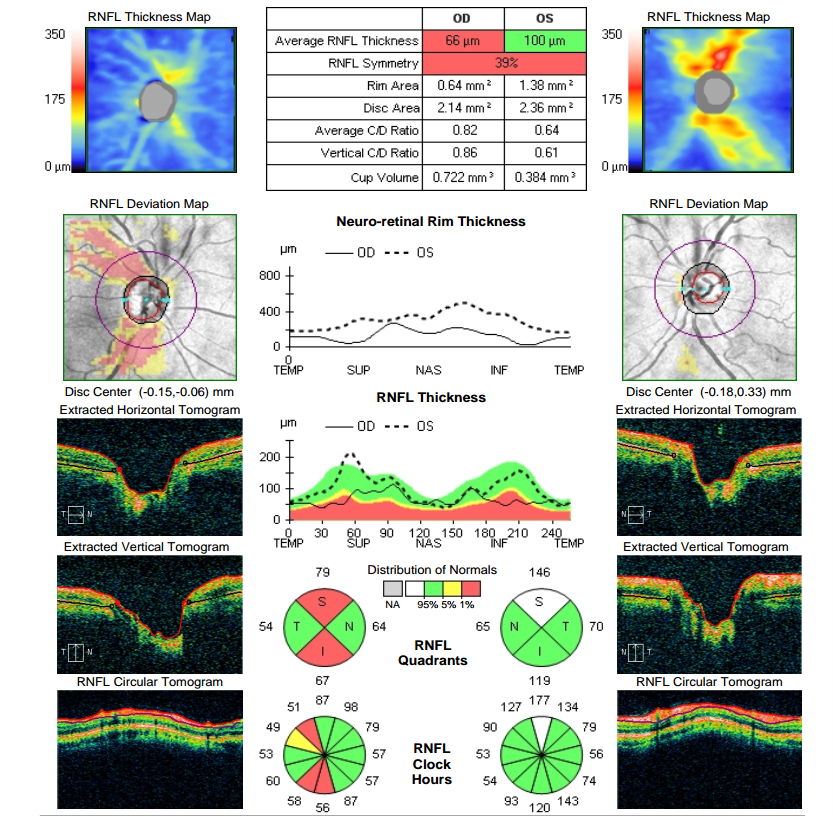
\includegraphics[width=\linewidth]{img/oct.png} 
                \caption{Exemplo de saída de um exame de OCT}
            \end{figure}
            
            
    \end{columns}
    
\end{frame}

\begin{frame}{Redes Neurais Convolucionais}

    \begin{figure}
        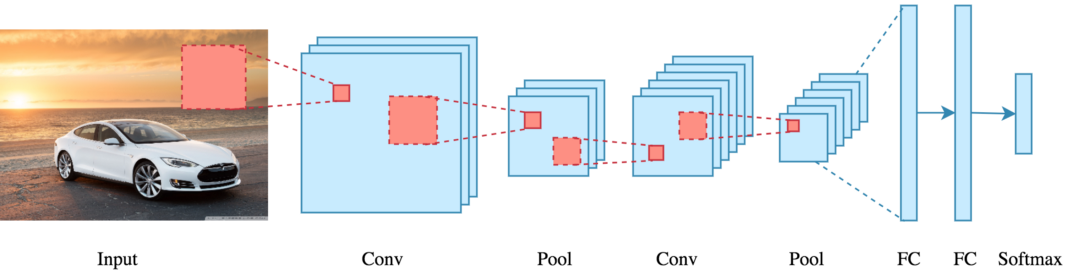
\includegraphics[width=4in]{img/convolucao.png} 
        \caption{Esquema de uma rede neural convolucional}
    \end{figure}
    
    \begin{figure}
        \centering

        \subfloat{%
          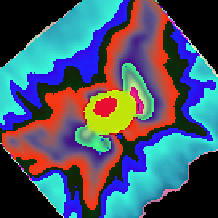
\includegraphics[scale=0.2]{img/vgg16/data.png}
          \label{fig:convolucao:data}
        }
        \subfloat{%
          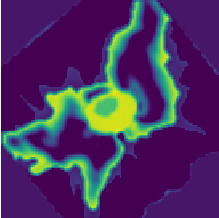
\includegraphics[scale=0.2]{img/vgg16/conv1_1.png}
          \label{fig:convolucao:conv11}
        }
        \subfloat{%
          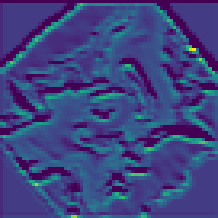
\includegraphics[scale=0.2]{img/vgg16/conv2_1.png}
          \label{fig:convolucao:conv21}
        }
        \subfloat{%
          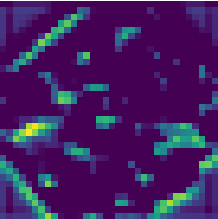
\includegraphics[scale=0.2]{img/vgg16/conv3_1.png}
          \label{fig:convolucao:conv31}
        }
        \subfloat{%
          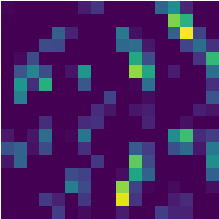
\includegraphics[scale=0.2]{img/vgg16/conv4_1.png}
          \label{fig:convolucao:conv41}
        }
        \subfloat{%
          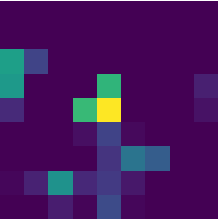
\includegraphics[scale=0.2]{img/vgg16/conv5_1.png}
          \label{fig:convolucao:conv51}
        }
        
        \caption{Saídas intermediárias da rede VGG16}
        \label{fig:intermediarias}
    \end{figure}
\end{frame}



\begin{frame}{Trabalhos relacionados}
    \begin{itemize}
        \item Estudos mostram a utilização de CNNs em oftalmologia
        \item Li et al (2017) fizeram a classificação de retinopatia diabética utilizando CNNs com transfer learning 
        % \footnote{LI, X. et al. Convolutional neural networks based
        % transfer learning for diabetic retinopathy fundus image
        % classification. In: 2017 10th International Congress on
        % Image and Signal Processing, BioMedical Engineering and
        % Informatics (CISP-BMEI), 2017.
        % }
        \item Lee et al (2017) fizeram a classificação de degeneração macular em imagens de OCT com a CNN VGG16 
        % \footnote{LEE, C. S.; BAUGHMAN, D. M.; LEE, A. Y. Deep
        % learning is effective for classifying normal versus age-related
        % macular degeneration oct images. Ophthalmology Retina, v.
        % 1, n. 4, p. 322 – 327, 2017.
        % }
    \end{itemize}
    
\end{frame}



\begin{frame}{Trabalho desenvolvido}

    \begin{columns}
        \column{0.6\textwidth}

            \begin{itemize}
                \item Rede VGG16
                \item Classificação de pacientes em glaucoma e normal
                \item Imagens de espessura de camada de fibras nervosas
                \item Utilização de técnica de transfer learning
                \item 9800 imagens no dataset de treinamento
                \item 24 imagens no dataset de validação
                \item Framework de deep learning utilizado: Caffe
            \end{itemize}

        \column{0.4\textwidth}

        \begin{figure}
            \centering
    
            \subfloat{%
              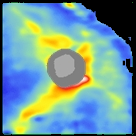
\includegraphics[scale=0.35]{img/ex/p0061_0.png}
            }\qquad
            \subfloat{%
              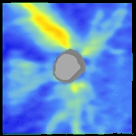
\includegraphics[scale=0.35]{img/ex/p0005_0.png}
            }\qquad
            \subfloat{%
              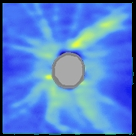
\includegraphics[scale=0.35]{img/ex/p0009_0.png}
            }\qquad
            \subfloat{%
              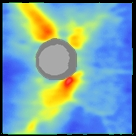
\includegraphics[scale=0.35]{img/ex/p0062_0.png}
            }
            
            \caption{Exemplos de treinamento}
        \end{figure}
        
    \end{columns}
    
    
    
\end{frame}

\begin{frame}{Resultados e discussões}
    \begin{columns}
		\column{0.5\textwidth}
            \begin{itemize}
                \item Acurácia final de 95.8\%
                \item Alto erro no dataset de validação
                \item Necessária utilização de técnicas para aumentar o dataset artificialmente
                \item 5000 iterações
                \item 1h de processamento
            \end{itemize}
		
        \column{0.5\textwidth}
            \begin{figure}
                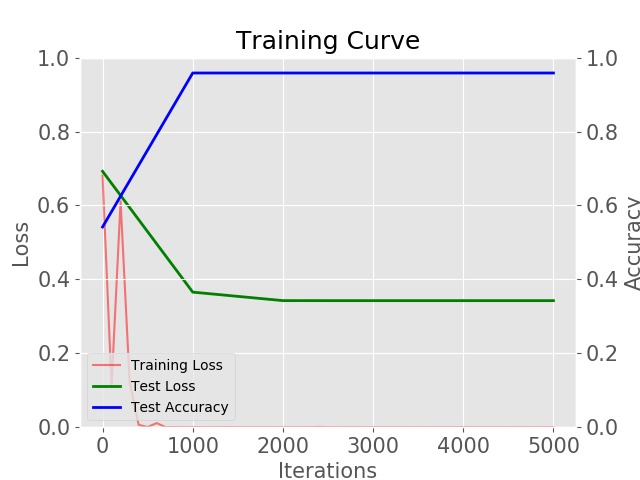
\includegraphics[width=\linewidth]{img/curve_vgg16.png}
                \caption{Evolução de acurácia e erro de treino e validação} 
            \end{figure}            
            
    \end{columns}
    
\end{frame}

\begin{frame}{Conclusão e próximos passos}
    \begin{itemize}
        \item Diagnóstico de glaucoma a partir de imagens de OCT é viável
        \item Possível ocorrência de overfitting devido à pequena quantidade de imagens no dataset de treino
        \item Novos experimentos com conjunto estendido de imagens já em preparação
    \end{itemize}
\end{frame}

\begin{frame}[focus]
    Obrigada pela atenção 
    \vfill
    {\small Samira J. Braga

    sjbraga@projesi.com.br}
\end{frame}

% \section{CNNs em oftalmologia}

% \section{Metodologia e desenvolvimento}



\end{document}
